\subsection{Modele danych}
Dane użytkownika, zapisywane w aplikacji można sklasyfikować jako forma \enquote{notatek}.
Zdecydowano się nadać im modułowy charakter, pozwalając w ten sposób na wykorzystywanie różnych typów notacji muzycznej
w ramach określonego zbioru, który sumarycznie może opisywać aranżowany utwór.
Wykorzystano stąd dwupoziomowy podział obiektów.

Pierwszy poziom stanowi koncepcja
\enquote{zeszytu do nut} (dalej okeślanego pojęciem \enquote{zeszyt}), jako zbioru notatek reprezentowany przez encję Book.
Idąc dalej tym tokiem, przyjęto określenie \enquote{strona} jako encja Page,
odnoszące się do poziomu drugiego — pojedynczej notatki użytkownika.
Obie encje implementują prosty interfejs Entity, deklarujący pole id,
ułatwiając działanie serwisów zarządzających persystencją.

\begin{figure}[H]
	\begin{center}
		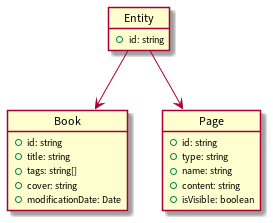
\includegraphics[scale=0.9]{media/Entity.png}
	\end{center}
	\caption{Modele encji implementujące interfejs Entity.}
	\label{rys:entity}
\end{figure}

Model encji Book zawiera pola: title — jako tytuł zeszytu, tags — przechowujące opisujące go słowa kluczowe,
cover — będące zapisem base64 \cite{64} zdjęcia, ustawionego jako okładka zeszytu, oraz automatycznie ustawiane modificationDate — wskazujące
na datę ostatniej modyfikacji zeszytu.
Model encji page zawiera pola: type — określające typ strony, name — zawierające jej nazwę, content — przechowujące zawartość oraz
isVisible — wyznaczające stan widoczności zawartości strony.
Zawartość strony jest zapisywana jako tekst lub w przypadku zawartości multimedialnej — w formacie base64 \cite{64}.

Identyfikatory encji są tworzone uniformowo, jako sygnatura czasowa systemu Unix, w momencie utworzenia obiektu.
Synchroniczność realizowanych przez aplikację akcji tworzących instacje obiektów gwarantuje unikatowość identyfikatorów
występujących w bazie.
Po utworzeniu obiektu jego identyfikator nie podlega modyfikacji.

Jako wyznacznik zależności między encjami Book i Page, w bazie przechowywana jest dotatkowo tablica obiektów Index.
Z uwagi na jej nadrzędny charakter, nie implementuje ona od interfejsu Entity. Występuje w bazie pojedynczo, pod ustalonym
kluczem \enquote{INDEX}.

\begin{figure}[H]
	\begin{center}
		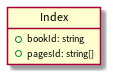
\includegraphics[scale=0.9]{media/Index.png}
	\end{center}
	\caption{Model obiektu Index.}
	\label{rys:index}
\end{figure}

\subsection{Diagramy przepływu}
Diagram UX (ang. user flow experience) oddaje założenia dotyczące przebiegu \enquote{doświadczeń użytkownika} (ang. user experience || UX)
w ramach projektowanej aplikacji. Na podstawie przyjętych konwencji dotyczących nazewnictwa oraz założeń projektowych,
można zobrazować planowane działanie aplikacji z punktu widzenia jej użytkownika:

\begin{figure}[H]
	\begin{center}
		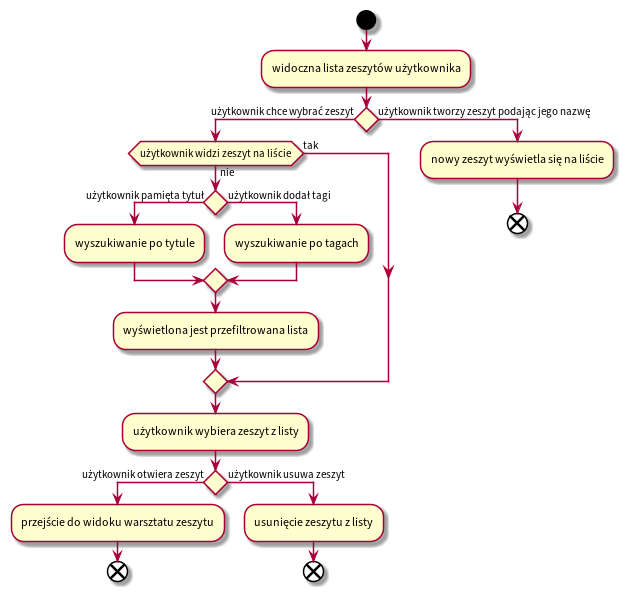
\includegraphics[scale=0.5]{media/UserFlowLibrary.png}
	\end{center}
	\caption{Diagram przepływu dla widoku biblioteki zeszytów użytkownika.}
	\label{rys:flow-library}
\end{figure}
\begin{figure}[H]
	\begin{center}
		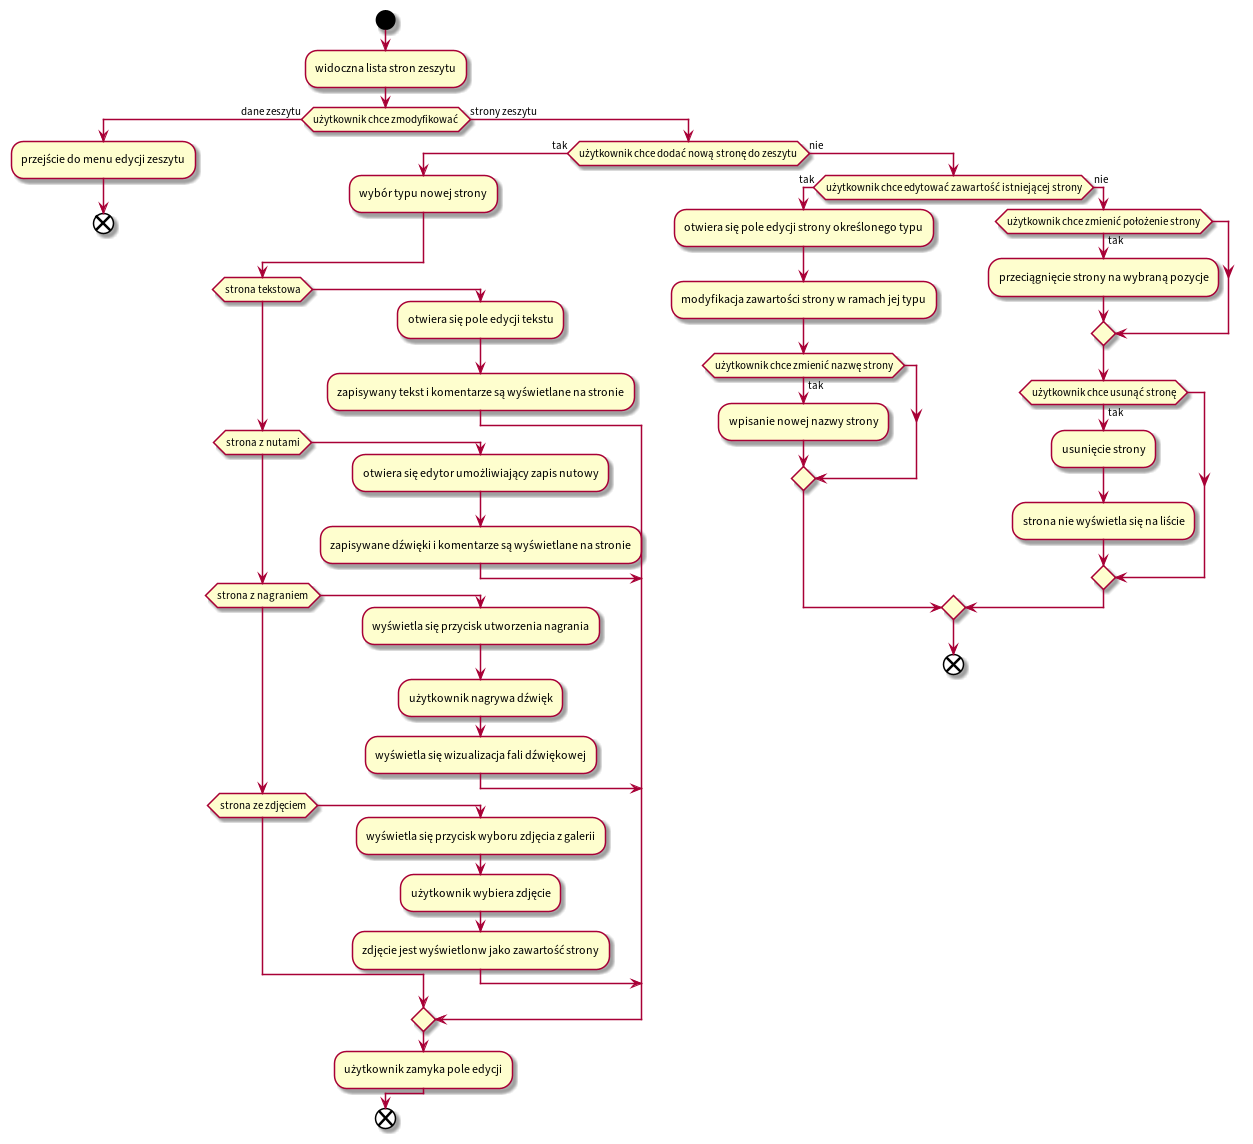
\includegraphics[scale=0.36]{media/UserFlowWorkshop.png}
	\end{center}
	\caption{Diagram przepływu dla widoku warsztatu użytkownika.}
	\label{rys:flow-workshop}
\end{figure}
\begin{figure}[H]
	\begin{center}
		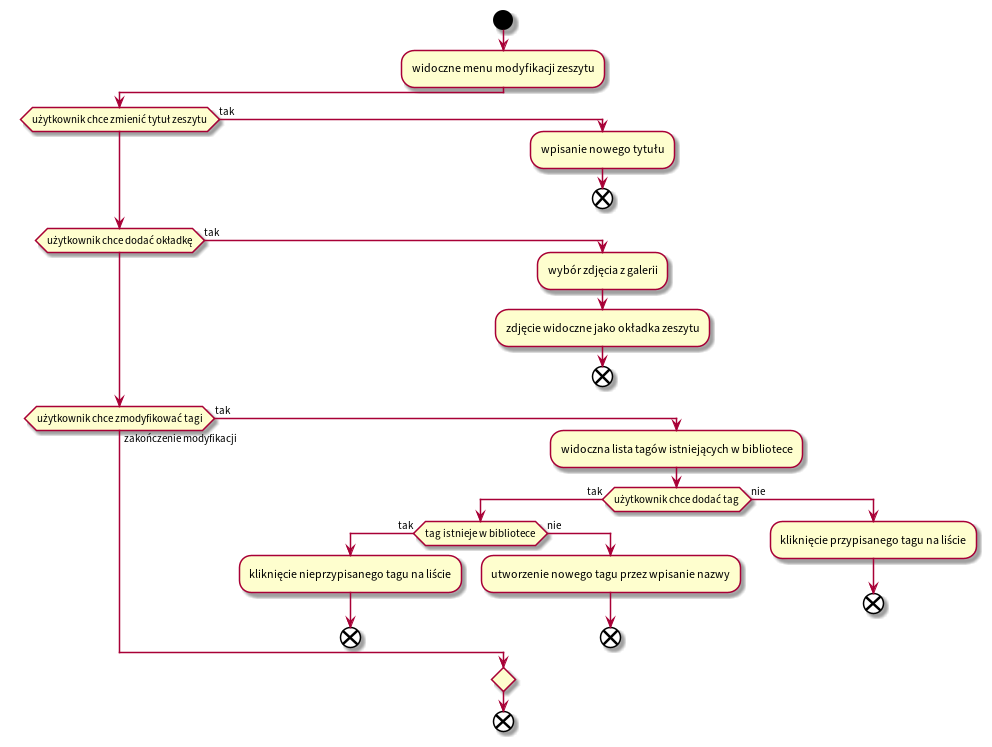
\includegraphics[scale=0.4]{media/UserFlowBook.png}
	\end{center}
	\caption{Diagram przepływu dla menu edycji zeszytu.}
	\label{rys:flow-book-menu}
\end{figure}

\subsection{Architektura aplikacji}
Jako model architektury aplikacji przyjęto architekturę warstwową. Pozwala ona odseparować zadania wykonywane przez
poszczególne komponenty aplikacji, ułatwiając utrzymanie kodu. Jest to osiągane poprzez rozgraniczenie zadań
realizowanych przez poszczególne warstwy. Architektura warstwowa charakteryzuje się hierarchicznym układem komponentów,
co przekłada się na zwiększenie przejrzystości kodu. W ramach projektu zastosowano trzy warstwy podziału:

\begin{itemize}
	\item Warstwa prezentacji — realizowana przez komponenty Vue, stanowiące interfejs użytkownika. Wykonuje podstawowe operacje
	      jak obsługa wtyczek do wizualizacji elementów lub funkcje formatowania tekstu.
	\item Warstwa logiki biznesowej — obejmująca szczególnie serwisy zarządzania stanem aplikacji, stanowiące punkt wykonania
	      akcji podejmowanych przez użytkownika. Odnosi się do danych pobieranych z bazy.
	\item Warstwa dostępu do danych — odpowiadająca za komunikacje z bazą danych, w oparciu o model encji. Przekazuje
	      dane modyfikowane w warstwie logiki biznesowej, zapewniając ich trwałość.
\end{itemize}

\begin{figure}[H]
	\begin{center}
		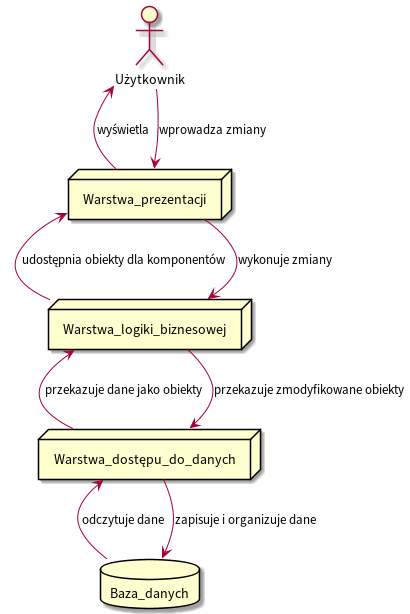
\includegraphics[scale=0.7]{media/Architecture.png}
	\end{center}
	\caption{Diagram realizacji architektury warstwowej.}
	\label{rys:architecture}
\end{figure}

Serwisy warstwy logiki biznesowej komunikują się z serwisami warstwy dostępu do danych.
Otrzymują w ten sposób obiekty notatek, zapisane trwale w pamięci urządzenia.
Odczytane obiekty są traktowane jako \textit{stan} danego serwisu w ujęciu globalnym — stąd sumarycznie: \textit{stan aplikacji}.
Dzięki temu komponenty Vue warstwy prezentacji mogą z nich korzystać — wyświetlając je oraz umożliwiając edycję.
Wprowadzanie zmian należy z powrotem do zadań warstwy logiki biznesowej. Obserwacja zmian \textit{stanów} serwisów tej warstwy
pozwala odzwierciedlić je w bazie danych.

Ma to miejsce na dwóch płaszczyznach: (1) w przypadku modyfikacji danych obiektu,
odpowiedzialność trwałego zapisu zmienionego obiektu przekazywana jest do PersistencyService;
(2) w przypadku modyfikacji przynależności obiektu — jako akcji
tworzenia i usuwania zeszytów oraz stron — zapis zmian realizowany jest w koordynacji z serwisem Indexer.
Taki rozdział zadań daje możliwość kontroli akcji podejmowanych przez użytkownika, co pozwala uniknąć nieoczekiwanych
zdarzenień podczas działania aplikacji — mogących doprowadzić do błędów.

\begin{figure}[H]
	\begin{center}
		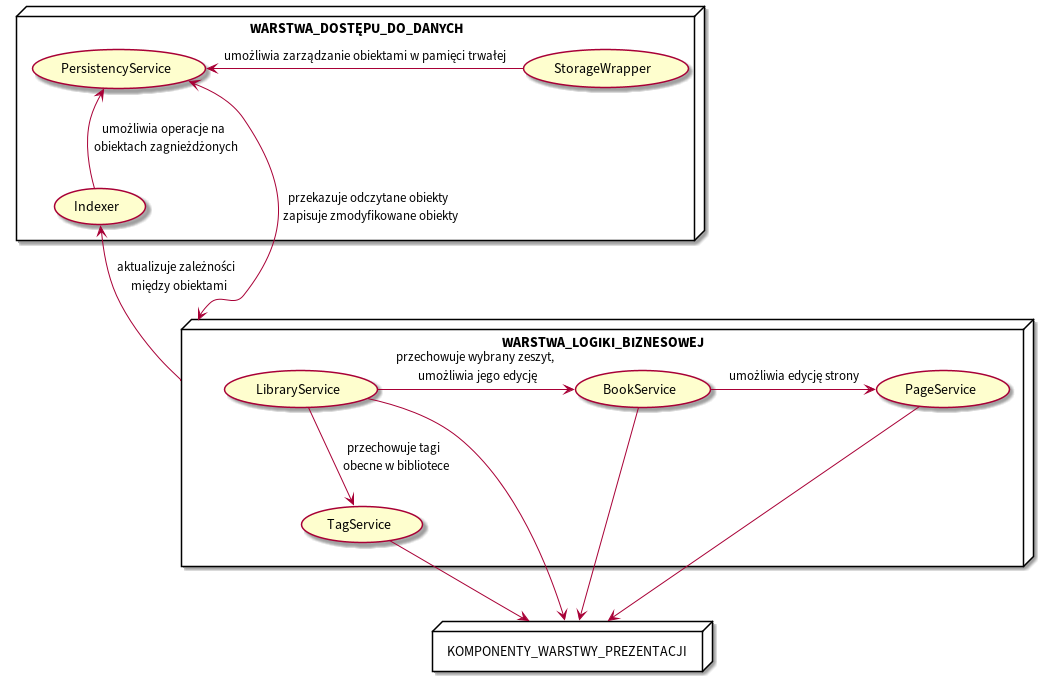
\includegraphics[scale=0.4]{media/LayerComunication.png}
	\end{center}
	\caption{Diagram przedstawiający komunikację między serwisami warstw aplikacji.}
	\label{rys:layer-communication}
\end{figure}

\subsection{Warstwa dostępu do danych}
W aplikacji zastosowano bazę danych typu klucz-wartość Ionic Storage \cite{storage}. Aby umożliwić
zarządzanie obiektami zagnieżdżonymi — jako: \textit{zeszyt} zawierać może wiele \textit{stron} — przy zachowaniu
niezależności operacji na obiektach, zastosowano trzy serwisy:

\begin{itemize}
	\item StorageWrapper

	      Z uwagi na charakter kluczy i wartości bazy — jako dwóch ciągów znaków — obiekty zapisywane w bazie są
	      konwertowane do ciągów JSON \cite{json}. StorageWrapper \textit{opakowuje} bibliotekę Ionic Storage, udostępniając podstawowe
	      metody zarządzania danymi oraz konwertując przetwarzane dane na ciągi znaków JSON i odwrotnie.
	      Jako jedyny bezpośrednio korzysta z metod oferowanych przez Ionic Storage \cite{storage}.
	\item PersistencyService

	      Z serwisu StorageWrapper korzysta PersistencyService,
	      wykorzystujący jego funkcje w kontekście konkretnych obiektów.
	      Zawiera logikę wykorzystującą interfejs Entity, implementowany przez encje Book i Page. Odwołuje się do danych
	      serwisu Indexer celem identyfikacji i lokalizacji obiektów zapisanych w bazie.
	\item Indexer

	      Poza encjami Book i Page przechowywana jest również tablica obiektów Index określająca
	      zależności między encjami, za którą odpowiada serwis Indexer.
	      Jego stan początkowy jest wczytywany z bazy przy uruchomieniu aplikacji.
	      Informacje o zmianach są sygnalizowane przez serwisy warstwy logiki biznesowej.
	      Odpowiadając na nie, serwis Indexer zapewnia zgodność tablicy indeksów ze stanem rzeczywistym
	      biblioteki użytkownika. W pewnym stopniu emuluje on możliwości relacyjnej bazy danych.
\end{itemize}

\begin{figure}[H]
	\begin{center}
		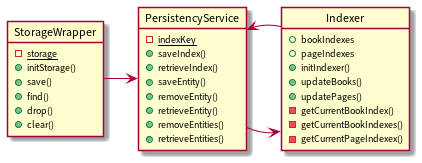
\includegraphics[scale=0.9]{media/PersistencyLayer.png}
	\end{center}
	\caption{Serwisy warstwy dostępu do danych.}
	\label{rys:persistency-layer}
\end{figure}

\subsection{Warstwa logiki biznesowej}
Warstwę logiki biznesowej stanowią serwisy zarządzania stanem aplikacji.
Wszystkie opierają się na bibliotece Pinia.
Umożliwia to funkcjonowanie niezależne od komponentów Vue budujących interfejs aplikacji,
udostępniając dla nich globalny stan, do którego mogą się odwoływać.

Aby rozdzielić zadania tej warstwy, serwisy zostały podzielone według domen:
\begin{itemize}
	\item LibraryService — odpowiada za zarządzanie biblioteką zeszytów użytkownika.
	\item TagService — udostępnia zbiór tagów utworzonych w ramach biblioteki użytkownika, umożliwiając efektywną kategoryzację zasobów.
	\item BookService — odpowiada za wprowadzanie zmian w kontekście zeszytu: jego danych oraz zawartości.
	\item PageService — odpowiada za edycję stron wybranego zeszytu.
\end{itemize}

\begin{figure}[H]
	\begin{center}
		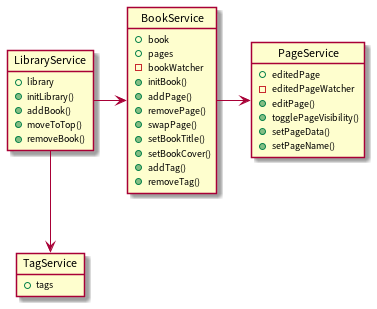
\includegraphics[scale=0.9]{media/LogicLayer.png}
	\end{center}
	\caption{Serwisy warstwy logiki biznesowej.}
	\label{rys:logic-layer}
\end{figure}


\subsection{Warstwa prezentacji}
\subsubsection{Projekt interfejsu}
Współgrając z dwupoziomową strukturą modelu danych, projekt interfejsu obejmuje dwa widoki: widok biblioteki i widok warsztatu.
Są one wspierane przez komponenty główne w postaci oferowanych przez Ionic Framework modali oraz menu \cite{ionic},
rozszerzających funkcjonalności aplikacji.

Czerpiąc inspirację ze współczesnych, popularnych koncepcji projektowania interfejsów
opartych o modułowość, wizualizacja tworzonych przez użytkownika notatek realizowana jest przez komponenty
kart (tu: oferowanych przez Ionic Framework \cite{ionic}). Podobne rozwiązania stosowane są w przytoczonych
w części teoretycznej
aplikacjach — m.in. w Notion \cite{notion}.
Karty szczególnie dobrze sprawdzają się enkapsulując zawartości niewielkich rozmiarów.
Ich zastosowanie wizualnie oddziela od siebie poszczególne moduły.
Z tych powodów przyjęto je jako kluczowe elementy kompozycji aplikacji — nadające kształt zeszytom oraz stronom.

Do edycji składu lub zawartości modułów reprezentowanych przez karty wykorzystano komponenty wysuwanych od dołu ekranu modali \cite{ionic}.
Pozwalają one śledzić proces edycji na bieżąco — zajmując jedynie część ekranu, nie przysłaniają edytowanych kart.
Polepsza to również odczucie responsywności aplikacji.
Zastosowano również menu \cite{ionic}, jako komponent dodatkowy, stanowiący przestrzeń edycji danych wybranego zeszytu. Proces ten zwykle
nie odnosi się do innych elementów kolekcji, dlatego może być w ten sposób odseparowany od kontekstu.

Widok biblioteki umożliwia wizualizację kolekcji zeszytów użytkownika. Na kartach przedstawiających zeszyty widoczny jest tytuł,
data modyfikacji oraz przypisane tagi. Jeżeli użytkownik doda do zeszytu okładkę, ułatwiającą identyfikację zeszytu w kolekcji — zostanie
tu wyświetlona. Widok biblioteki umożliwia podstawowo trzy akcje: (1) Dodawanie zeszytów, realizowane przez przycisk w dolnym rogu ekranu;
(2) Usuwanie zeszytów, po kliknięciu ikony usunięcia \cite{ionic} na określonej karcie;
(3) Otwieranie zeszytów — przejście do widoku zeszytu, po kliknięciu dowolnego miejsca karty (ikona strzałki \cite{ionic}
ma jedynie znaczenie symboliczne).

Możliwość filtracji zeszytów realizowana jest przez modal, otwierany po kliknięciu górnego paska widoku biblioteki.
Użytkownik może szukać zeszytów po ich tytułach oraz po słowach kluczowych.

\begin{figure}[H]
	\begin{center}
		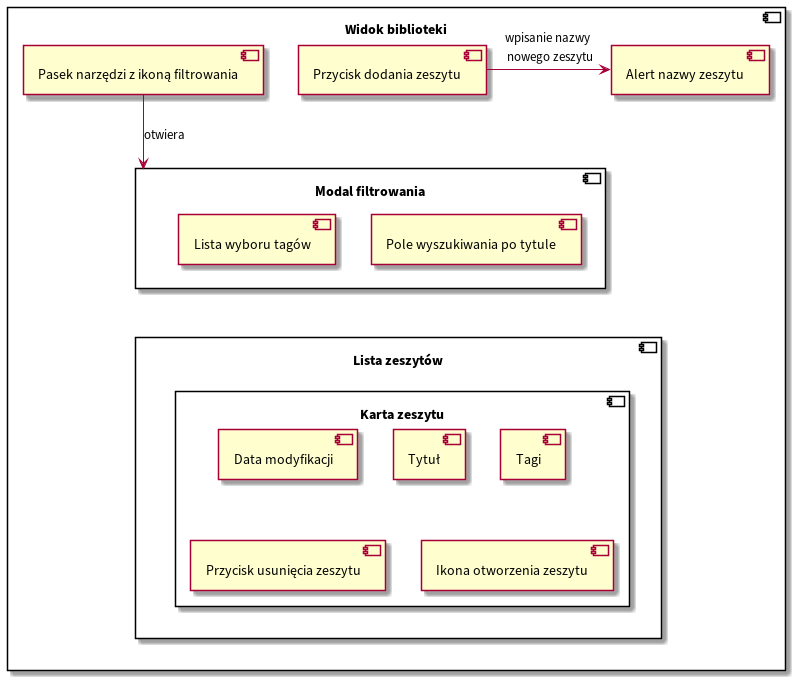
\includegraphics[scale=0.5]{media/LibraryInterface.png}
	\end{center}
	\caption{Diagram interfejsu widoku biblioteki.}
	\label{rys:library-interface}
\end{figure}

\begin{figure}[H]
	\begin{center}
		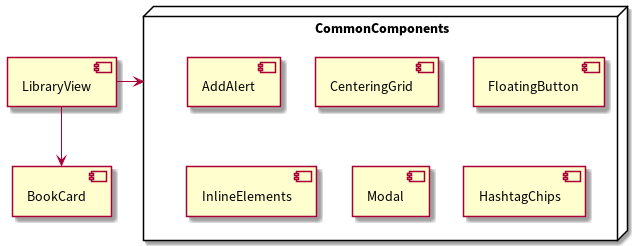
\includegraphics[scale=0.6]{media/LibraryComponents.png}
	\end{center}
	\caption{Drzewo komponentów Vue realizujących widok biblioteki.}
	\label{rys:library-components}
\end{figure}

Grupa komponentów wspólnych stanowi elementy, z których korzystają oba widoki — biblioteka i warsztat. Należą do nich:
AddAlert — umożliwiający dodanie elementu poprzez wpisanie jego nazwy, FloatingButton — obecny w postaci przycisku dodania elementu,
a także komponenty odpowiadające za przypisanie określonego stylu komponentom w nich zagnieżdżonych.

Widok warsztatu umożliwia wizualizację i edycję zawartości zeszytu. Przycisk w rogu ekranu pozwala dodać stronę do zeszytu.
Po dodaniu jest ona reprezentowana przez komponent karty. Zawartość strony może zostać ukryta,
przy użyciu przycisku z ikoną oka \cite{ionic}. Przytrzymanie przycisku powoduje trwałe usunięcie strony, sygnalizowane wibracją urządzenia.
Strona zawiera także przycisk umożliwiający jej przemieszczenie względem pozostałych stron. Jest to realizowane przy użyciu
biblioteki SortableJS \cite{sortablejs}.
W tym miejscu wyświetla się także nazwa
strony, jeżeli została nadana przez użytkownika.

Możliwość edycji strony realizowana jest przez modal, otwierany po kliknięciu ikony plusa \cite{ionic}. Zawartość modalu zależy od
typu edytowanej strony, zawierając stosowny interfejs edycji zawartości. Każdej stronie można tu również przypisać nazwę.

Modyfikacja danych zeszytu umożliwiana jest przez menu, otwierane przy kliknięciu górnego paska widoku zeszytu.
Przycisk z ikoną zdjęcia \cite{ionic} umożliwia dodanie okładki; kliknięcie symbolu zakładki pozwala przypisać słowo kluczowe
do zeszytu. Można w tym miejscu również zmienić tytuł zeszytu.

\begin{figure}[H]
	\begin{center}
		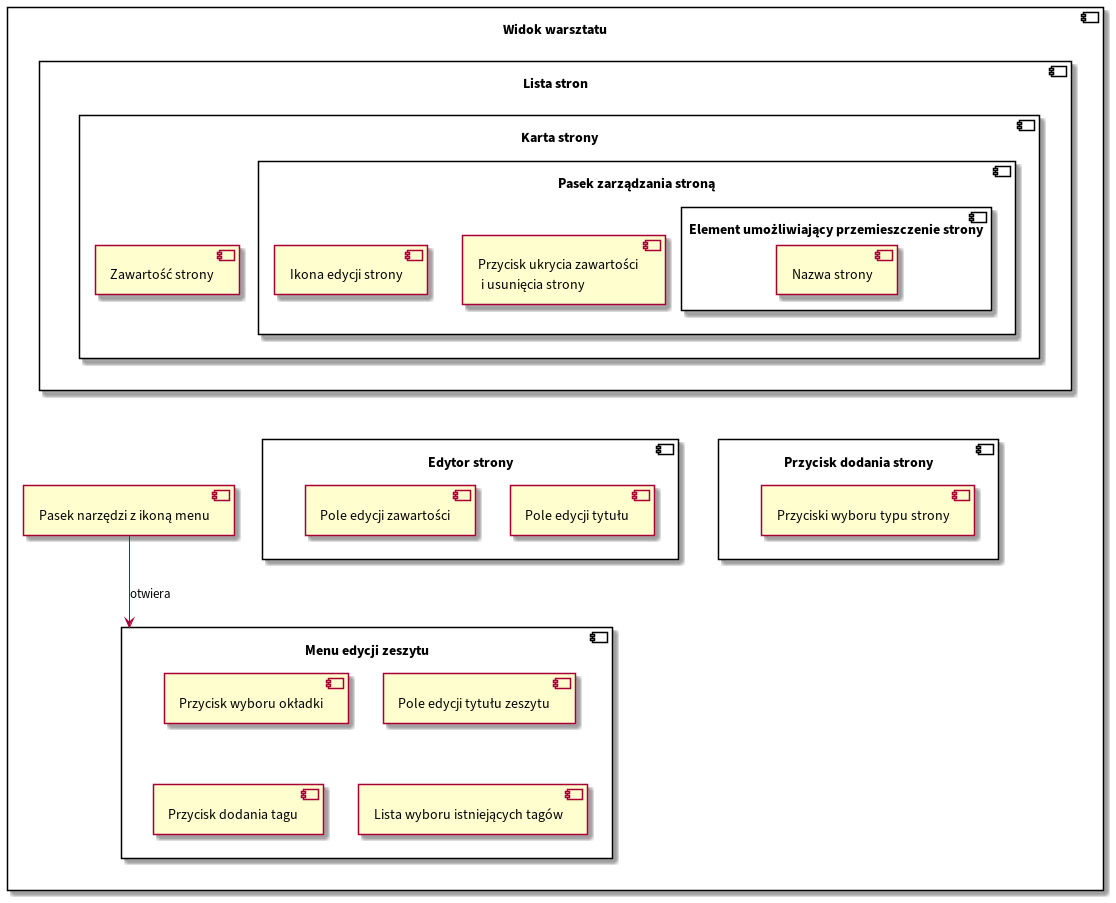
\includegraphics[scale=0.4]{media/WorkshopInterface.png}
	\end{center}
	\caption{Diagram interfejsu widoku warsztatu.}
	\label{rys:workshop-interface}
\end{figure}

\begin{figure}[H]
	\begin{center}
		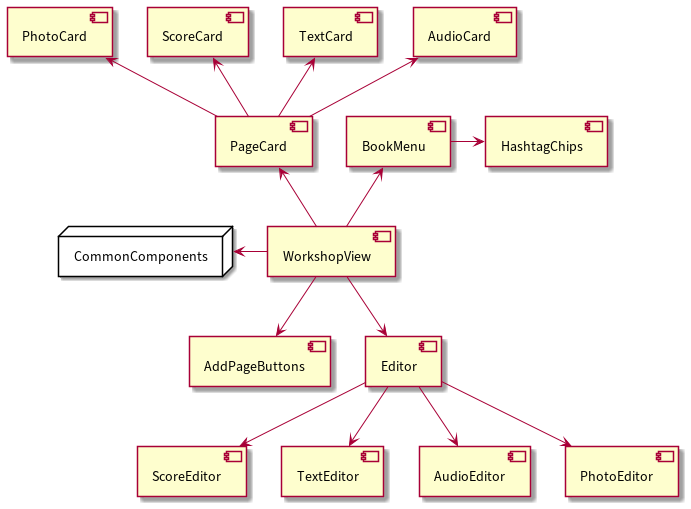
\includegraphics[scale=0.6]{media/WorkshopComponents.png}
	\end{center}
	\caption{Drzewo komponentów Vue realizujących widoku zeszytu.}
	\label{rys:workshop-components}
\end{figure}

\subsubsection{Implementacja funkcjonalności wspierających aranżację}
Przedstawione wcześniej komponenty stanowią \enquote{środowisko}, które umożliwia implementację konkretnych funkcjonalności
wspierających proces aranżacji muzycznej. Realizowane są one przez podział stron na cztery — zdefiniowane w wymaganiach aplikacji — typy.
Charakteryzują się one odmiennym rodzajem wizualizacji oraz zróżnicowanym procesem edycji. Aby to umożliwić, komponenty główne
dopasowują dynamicznie komponenty odpowiadające za wizualizację i edycję stron w zależności od ich typu.
Dynamiczne dopasowanie jest realizowane dzięki zastosowaniu component-is oferowanego przez Vue \cite{vue}.

Komponenty wizualizacji i edycji tekstu obsługują notatki tekstowe, umożliwiając dodawanie subtelnych (jako: nieodwracających uwagi)
komentarzy. Podczas edycji użytkownik zapisuje notatkę w polu tekstowym \cite{ionic}. Linijka tekstu poprzedzona symbolem \enquote{@} traktowana jest
jako komentarz. Aby ułatwić tworzenie komentarzy, układ klawiatury przy edycji treści takiej strony ustawiony jest na tryb \textit{e-mail} \cite{ionic}.
Komentarze wyświetlane są przy prawej krawędzi strony, mniej wyrazistą czcionką.

Wizualizacja zapisu nutowego realizowana jest przy użyciu biblioteki abcjs \cite{abcjs}. W ramach komponentu umożliwiającego edycję
użytkownik znów zapisuje notatkę w polu tekstowym, lecz jest ona renderowana jako zapis nutowy w komponencie strony.
Pomocna jest tu forma modala,
gdyż umożliwiaja on śledzenie zmian zapisu nutowego podczas jego edycji. Z uwagi na przystępną zasadę działania biblioteki
abcjs — za sprawą stosowania nazw literowych do określania nut, implementacja edytorów nut nie jest wymagana.
Każda strona o tym typie jest domyślnie inicjalizowana wartościami renderującymi kluczowe elementy notacji muzycznej.
Jednocześnie należy zwrócić uwagę, iż użytkownik potrzebujący szerszych możliwości edytora nutowego, powinien zaznajomić
się z dodatkowymi funkcjami oferowanymi przez abcjs.

Komponent edycji notatek dźwiękowych wykorzystuje do działania wtyczkę capacitor-voice-recorder \cite{vr}. Pozwala ona nagrać
dźwięk, korzystając z mikrofonu urządzenia. Po nagraniu użytkownik może ponownie edytować zawartość strony, zastępując
wcześniejszy zapis dźwiękowy nowym nagraniem. Wizualizacja fali dźwiękowej, realizowana przez bibliotekę wavesurfer.js \cite{wavesurfer}.
Umożliwia to orientację w jej przebiegu oraz odtwarzanie nagrania od wybranego momentu.

Możliwość użycia zdjęcia jako notatki realizowana jest przez wtyczkę capacitor-file-picker \cite{plugins},
pozwalającej wybrać plik (tu: zdjęcie) z pamięci urządzenia. Wybrane zdjęcie jest wyświetlane jako zawartość strony.
Edycja strony polega na możliwości zmiany wybranego zdjęcia.

\subsection{Continous Integration i Continous Delivery}
Przeprowadzenie procesu budowy aplikacji i generowania pliku instalacyjnego APK dla platformy Android jest realizowane przez aplikację
Buddy CI/CD \cite{buddy}. Umożliwia to automatyzację tych zadań, przyspieszając proces powstawania aplikacji.
W serwise zastosowano pojedynczy pipeline, który wykonuje następujący algorytm:

\begin{figure}[H]
	\begin{center}
		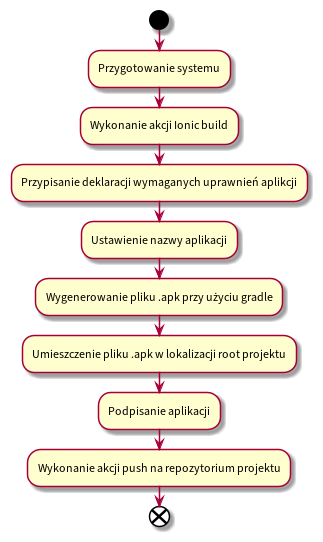
\includegraphics[scale=0.6]{media/ContinousDelivery.png}
	\end{center}
	\caption{Algorytm Continous Delivery realizowany przez Buddy CI/CD.}
	\label{rys:continous-delivery}
\end{figure}

Po przygotowaniu systemu pipeline projekt jest budowany przy użyciu Ionic \cite{ionic} oraz Capacitor \cite{capacitor},
do wyjściowego projektu platformy mobilnej.
Zadeklarowane w osobnym pliku wymagane uprawnienia aplikacji, pozwalające m.in. na korzystanie z mikrofonu urządzenia, są
przenoszone do projektu. Wówczas ustawiana jest nazwa wyjściowego pliku instalacyjnego APK.
Za jego budowę odpowiada akcja oparta o Gradle \cite{gradle}. Powstały w ten sposób instalacyjny aplikacji
jest przenoszony do lokalizacji root projektu, podpisywany certyfikatem oraz publikowany na repozytorium GitHub \cite{github}
przez akcję push.

Została przygotowana także poglądowa implementacja testów jednostkowych, przy użyciu biblioteki Jest \cite{jest}.
Testowaniu podlega serwis pomocniczy ArrayHelper udostępniający metody modyfikacji tablic.
Przebieg algorytmu testów można przedstawić za pomocą diagramu:

\begin{figure}[H]
	\begin{center}
		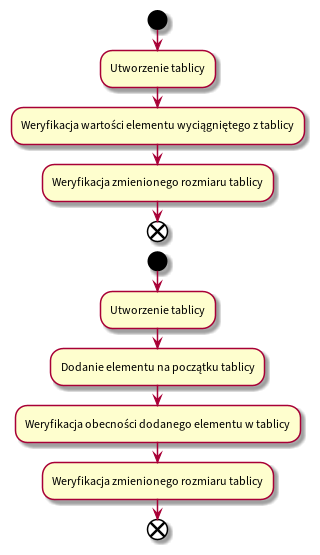
\includegraphics[scale=0.6]{media/ContinousIntegration.png}
	\end{center}
	\caption{Algorytm testów w ramach Continous Integration realizowany przez Buddy CI/CD.}
	\label{rys:continous-integration}
\end{figure}

Algorytmy Countinous Integration i Continous Development zostały zrealizowane w konwencji IAC \cite{iac}, w pliku YAML \cite{yaml}.